\chapter{Methoden und Techniken} \label{cha:Methoden}
    In diesem Kapitel geht es um die grundlegenden Bedingungen zur Untersuchung von Molekülen auf antiferromagnnetischen Oberflächen.
    Dazu gehört zunächst das Ultrahochvakuum, welches notwendig ist um eine saubere und wohl definierte Oberfläche zu erhalten.
    Ferner wird die Methode Beugung niederenergetischer Elektronen erläutert, womit auf die geometrische Struktur der Oberfläche geschlossen werden kann.
    Anschließend geht es um die Photoelektronenspektroskopie und ihre Teilbereiche, welche eine Untersuchung der elektronischen Struktur zulässt.

    \section{Grundlegende Bedingungen} \label{sec:Grundlagen}
        Um sich Oberflächen genauer anzusehen muss zunächst verhindert werden, dass sich keine unerwünschten Teilchen auf der Oberfläche absetzen.
        Hierzu wird Ultrahochvakuum (UHV) eingesetzt.
        Da es keine Pumpe gibt, die direkt vom Atmosphärendruck bis in den UHV Bereichen kleiner \SI{1e-9}{\milli\bar} reicht, ist ein mehrstufiges Pumpsystem unabdingbar \cite{Henzler}.
        In dem vorliegenden Aufbau wird dies durch Turbomolekularpumpen mit vorgeschalteten Scrollpumpen realisert.
        Ferner werden diese durch Titansublimationspumpen sowie Ionenpumpen unterstützt.
        Diese tiefen Drücke sind erforderlich, da schon bei einem Druck von \SI{1e-6}{\milli\bar} die Oberfläche innerhalb von \SI{10}{\milli\second} zu \SI{1}{\percent} mit den im Restgas vorhandenen Teilchen bedeckt wäre~\cite{Henzler}.

        Es gibt auch die Möglichkeit gezielt Gase in die Präperationskammer zu leiten, in der die Proben für die anschließenden Messungen vorbereitet werden.
        Dies geschieht dann durch sogenannte Leckventiele.
        Ein Maß für die Oberflächenbedeckung ist die Einheit Langmuir \si{\langmuir}, welcher einer Dosis entspricht.
        Dabei ist $\SI{1}{\langmuir} = \SI{1}{\torr} \cdot \si{\micro\second}$ also etwa $\SI{1.33e-6}{\milli\bar} \cdot \si{\second}$.
        Hier wird zu Grunde gelegt, dass jedes auf die Oberfläche auftreffende Teilchen auch haften bleibt. 
        Die Oberfläche besäße also einen Haftkoeffizienten von \num{1}, was in der Realität so nicht vorkommt.

        Das Vakuum dient allerdings nicht nur der Reinheit der Probe, sondern auch das die später emittierten Elektronen auch den Raum durchdringen und den Analysator erreichen können.
        Andernfalls würden die Teilchen durch Streuung an anderen Teilchen abgebremst werden und somit Informationen verlieren.
        % Elektronen hätten bei einem Druck von xx bar nur eine Reichweite von \textbf{QUELLE, Zahlen}.
        Da es sich um die Untersuchung von Oberflächen handelt ist somit auch bei den Techniken auf die Oberflächensensitivität zu achten.
        Relevant wird damit die mittlere freie Weglänge der verwendeten Sonde.
        Als perfekte Sonden stellten sich die Elektronen heraus, ihre inelastische mittlere freie Weglänge ist in \autoref{fig:Weg} graphisch dargestellt.
        \begin{figure}
            \centering
            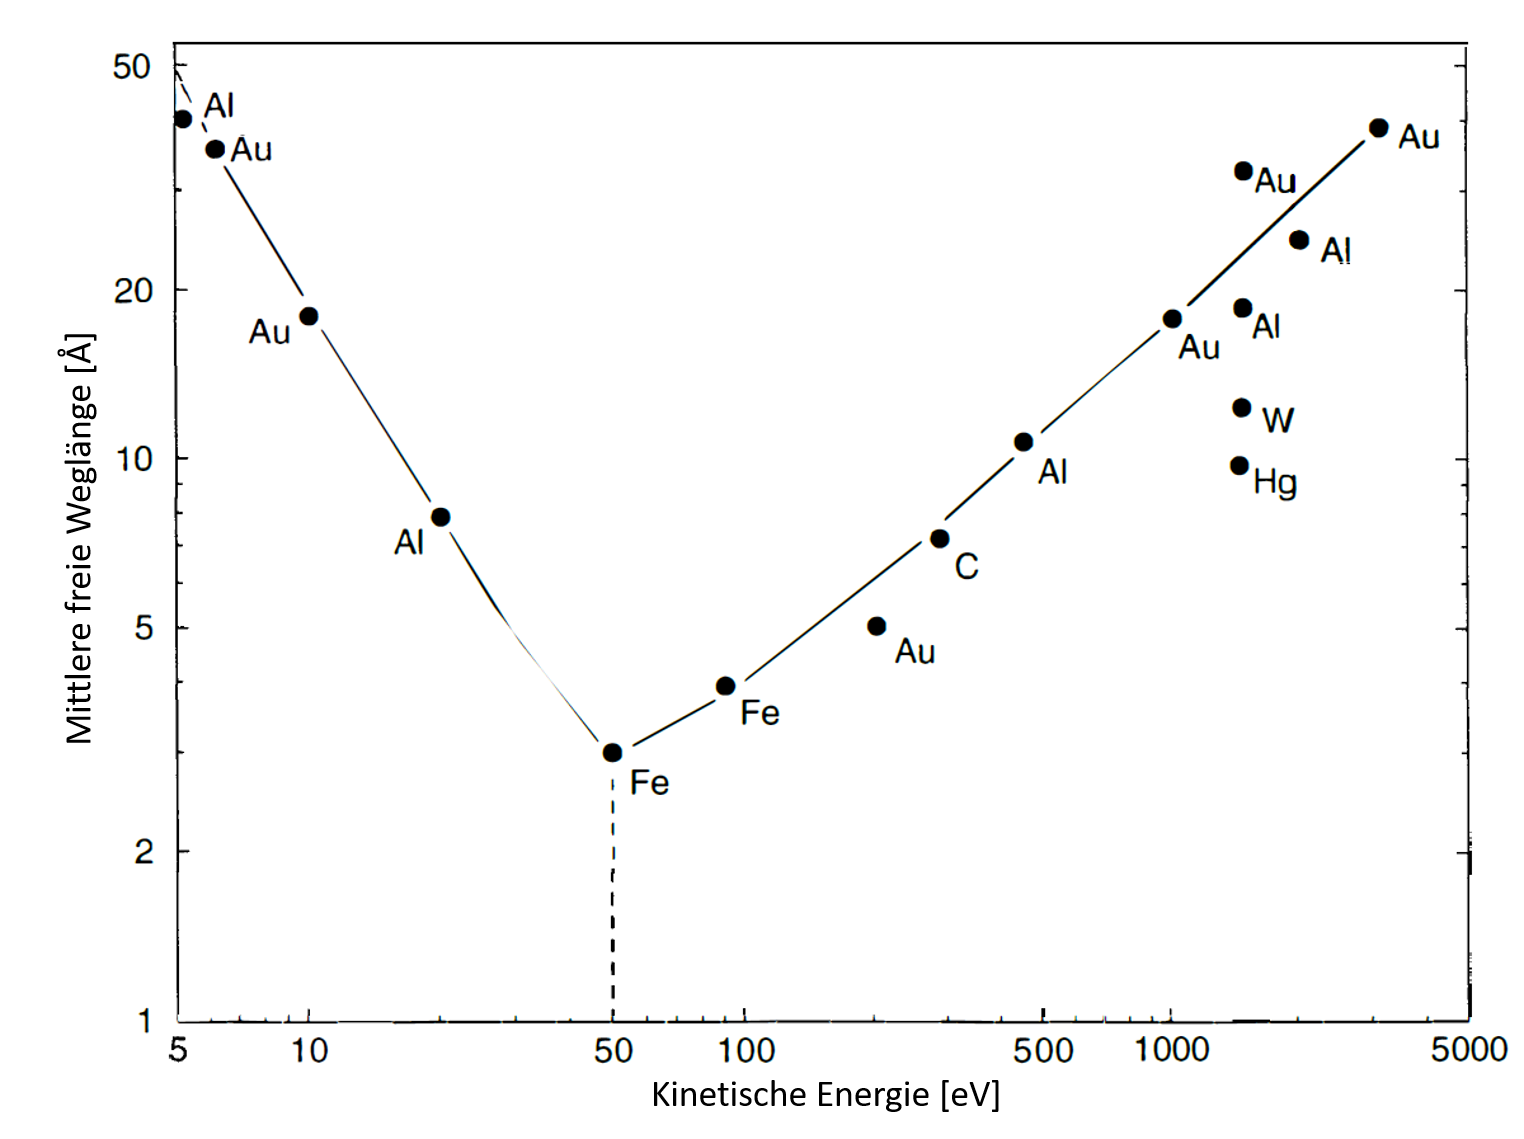
\includegraphics[width=0.7\textwidth]{./content/pictures/Weg}
            \caption{Die mittlere freie Weglänge für Elektronen in verschiedenen Materialien. Aus~\cite{Hüfner}.}
            \label{fig:Weg}
        \end{figure}
        Es ist zu erkennen, dass Elektronen mit einer kinetischen Energie im Bereich von \SIrange{30}{100}{\electronvolt} aus einer Tiefe von nicht mehr als \SI{5}{\angstrom} kommen.
        Werden also Elektronen als Sonden verwendet und ihre kinetische Energie angepasst, so kann davon ausgegagngen werden, dass sie nur aus Oberflächen nahen Bereichen kommen.

        Um Elektronen von der Probe kommend zu erhalten gibt es zwei Möglichkeiten.
        Zünächst können Elektronen in der Probe angeregt werden, die dann aus der Oberfläche austreten und detektiert werden können.
        Dies wird bei der Photoelektronenspektroskopie genutzt und in \autoref{sec:PES} genauer erläutert.
        Die zweite Möglichkeit ist es die Probe mit Elektronen im entsprechenden Energiebereich zu beschießen.
        Zurückkommenden Elektronen mit identischer kinetischen Energie können also nur aus Oberflächen nahen Bereichen kommen.
        Bei der Beugung niederenergetischer Elektronen wird dieses Prinzip verwendet und nun genauer beschrieben.

    \section{Beugung niederenergetischer Elektronen} \label{sec:LEED}
        \begin{figure}
            \centering
            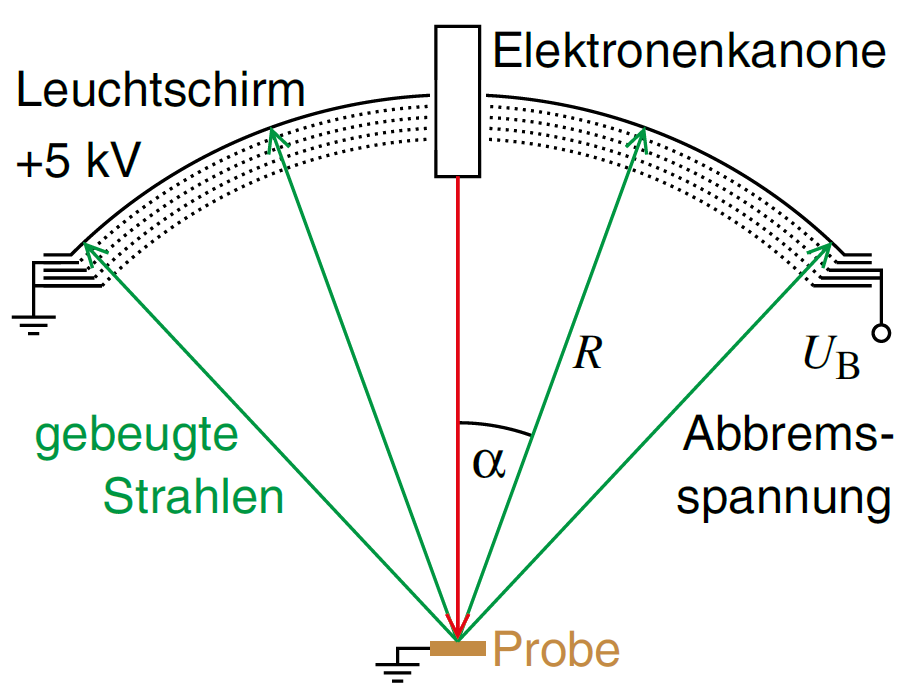
\includegraphics[width=0.5\textwidth]{./content/pictures/LEED}
            \caption{Innerer Aufbau der Optiken zur Beugung niederenergetischer Elektronen.
            Die Probe befindet sich im Zentrum des Schirms und auf Erdpotential, ebenso wie das erste und dritte Gitter.
            Die Abremsspannung liegt am zweiten Gitter an, am vierten Gitter die Beschleunigungsspannung.
            Aus~\cite{Fauster}.}
            \label{fig:LEED}
        \end{figure}
        Um sich die geometrische Oberflächenbeschaffenheit genau anzusehen wir die Beugung niederenergetischer Elektronen (\textit{Low energy electron diffraction}, LEED) eingesetzt.
        Hierbei werden Elektronen mit einer kinetischen Energie im Bereich der Oberflächensensitivität auf die Probe geschossen.
        Das entstehende Beugungsmuster ist charakteristisch für die Oberflächenbeschaffenheit und stellt die Oberfläche im reziproken Raum da.
        Der Aufbau mit seinen Optiken für die Beugung niederenergetischer Elektronen ist in \autoref{fig:LEED} abgebildet.
        
        Die Elektronen werden zunächst durch den Glühelektrischen Effekt erzeugt und durch einen Wehnelt-Zylinder gebündet.
        Diese beiden Komponenten bilden zusammen die Elektronenkanone.
        Anschließend werden Sie zur Probe hin beschleunigt, welche sich im Zentrum der Gitter befindet.
        Da die Probe geerdet ist geschieht dies durch eine negative Vorspannung zwischen Probe und Elektronenkanone.
        Die gestreuten Elektronen bewegen sich in alle Richtungen unter dem Winkel $\alpha$ zum senkrecht auftreffenden Elektronenstrahl von der Probe weg.
        Damit die Flugbahn nicht durch elektrische Felder beeinflusst wird befindet sich das erste von der Probe aus gesehen Netz ebenfalls auf Erdpotential.
        Genau der Vorspannung entsprechend wird durch das dahinter liegende Netz  ein elektrisches Feld aufgebaut, gegen das die Elektronen anlaufen.
        So können nur elastisch gestreute Elektronen die weiteren Netze durchlaufen.
        Das nächste Gitter liegt wieder auf Erdpotential, damit das vom dahinter liegenden Gitter erzeugte Beschleunigungsfeld nicht durchgreift.
        Dieses Beschleunigungsfeld wir durch eine hohe Spannung hervorgerufen und ist dafür notwendig, damit die Elektronen auf dem Leuchtschirm das Beugungsmuster erzeugen können.
        Mit Hilfe einer Kamera wird dieses Beugungsmuster erfasst ~\cite{Fauster}.

        Die Entstehung des Beugungsmusters geschieht durch Interferenz Effekte, es ist also eine periodische Struktur von Nöten.
        Ebenso muss damit die Wellenlänge der Elektronen im Größenbereich der Gitterkonstanten liegen.
        Folglich haben die Elektronen einer Energie zwischen \SIrange{30}{200}{\electronvolt}~\cite{oura_surface_2003}.
        Kinematisch betrachtet wird die Oberfläche von einer Primärwelle getroffen.
        Der von einem Streuer zurückgeworfene Anteil ohne zusätzliche Streuung interferiert mit den von anderen Streuen kommenden Sekundärwelle.
        Für elastisch gestreute Elektronen muss also für den Impuls gelten $\abs*{\vec{k}_\text{i}} = \abs*{\vec{k}_\text{f}}$.
        Intensitäten der einzelnen Spots $I$ ergeben sich dabei aus dem Formfaktor $F$ und dem Gitterfaktor $G$ zu
        \begin{equation}
            I = \abs*{F^2}\abs*{G^2}.
            \label{eqn:LEED}
        \end{equation}
        Mathematisch kommt der Formfaktor aus der Position und chemischen Natur der Atome innerhalb der Einheitszelle, wohingegen der Gitterfaktor die Periodizität der Gitters wiederspiegelt.
        Der Gitterfaktor ist nur ungleich Null, wenn die Lauebedingung erfüllt ist.
        Folglich darf der Impulsübertrag $\increment \vec{k}_{||}$ nur einen reziproken Gittervektor $\vec{g}_\text{hk}$ betragen, dies ist die Lauebedingung.
        Jeder Spot kann damit einem Impulsübertrag mit den Indizes $hk$ zugeordnet werden.
        Der Gitterfaktor gibt also nur Auskunft darüber ob ein Beugungsreflex auftaucht und wo, die Intensitäten hingegen werden rein durch den Formfaktor beschrieben.

        Da aber wie oben beschrieben die Impulserhaltung gelten muss und die Transaltionssymetrie senkrecht zur Oberfläche gebrochen ist ergibt sich für diese Komponente ein Impuls von $\vec{k}_{\text{f}\perp} = \pm \sqrt{\vec{k}_\text{i}^2 - (\vec{k}_{\text{i}||} + \vec{g}_\text{hk})^2}$.
        Positives Vorzeichen entspricht der Beugung in die Oberfläche hinein und negatives Vorzeichen für eine Beugung von der Oberfläche weg.
        $\vec{k}_{\text{f}\perp}$ kann auch imaginär werden, was zur Folge hat, dass keine Rückstreuung erfolgt.
        \begin{figure}
            \centering
            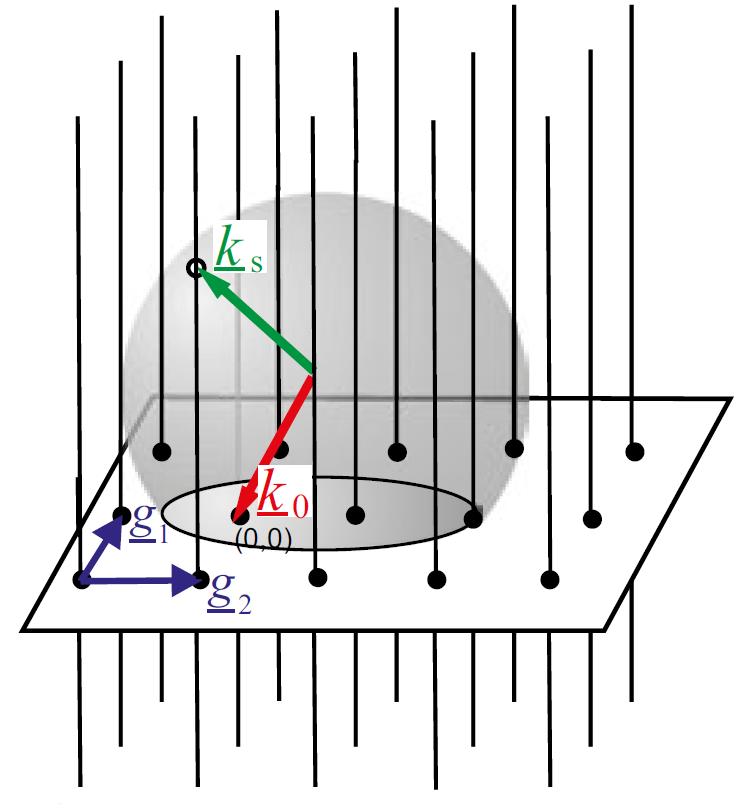
\includegraphics[width=0.4\textwidth]{./content/pictures/Ewald}
            \caption{Schamtische darstellung zur Veranschaulichung der Konstruktion der Ewaldkugel.
            Blaue Pfeile stellen die reziproken Gittervektoren da. 
            Der rote Pfeil den einfallenden Wellenvektor der Elektronen, grün den der gestreuten.
            Kopiert und modifiziert aus~\cite{Fauster}.}
            \label{fig:Ewald}
        \end{figure}
        Die Beugungsreflexe lassen sich für nahezu senkrechten Einfall mit Hilfe der Ewaldkugel konstruieren, veranschaulicht zu sehen in \autoref{fig:Ewald}.
        Hierzu wird das reziproke Gitter aufgespannt, es ergeben sich auf Grund der gebrochenen Symmetrie Gitterstangen.
        Um einen beliebiegen Startpunkt wird eine Kugel mit dem Radius $\vec{k}_\text{i}$ gezeichnet, so ergeben sich für alle schneidenen Gitterstangen der Kugel auch Beugungsreflexe.
        Der Schnittpunkt mit der Kugel zum Ursprung hin ergibt dann den gebeugten Wellenzahlvektor $\vec{k}_\text{f}$.

        % Größere Abstände im Realraum werden im reziproken Raum kleiner abgebildet.
        % Mit steigeneder Energie der Elektronen rücken die Beugungsmaxima dichter zum Zentrum hin.
        Die Annahme ohne Mehrfachstreuung der Elektronen ist zu einfach gefasst, weswegen lange keine Strukturanalyse mittels LEED möglich war.
        Ursache der Mehrfachstreuung ist der verhältnissmäßig große Streuquerschnitt der langsamen Elektronen an Atomen.
        Es kommt vermehrt zur Streuung mit den nächsten Nachbarn der Primär- wie auch Sekundärwelle, die sich wiederum gegenseitig beeinflussen.
        Tendenziell ist es möglich aus der Position der Beugungsreflexe auf die Größe der Einheitszelle zu schließen, durch Adsorbate und Domänen, kann dies allerdings erschwert werden.
        Werden die Intensitäten der Spots durch Variation der Energie aufgezeichnet ergeben sich charakteristische IV-Kurven.
        Ihre theoretische Berechnung ist sehr aufwendig, da sie den Formfaktor und zahlreiche Streueffekte berücksichtigen müssen.

    
    \section{Photoelektronenspektroskopie} \label{sec:PES}
        Die Grundlage ist der Photoelektronenspektroskopie ist der photoelektrische Effekt, der 1905 zum ersten Mal von Albert Einstein erklärt wurde~\cite{Einstein}.
        Hierbei werden Elektronen durch ein einfallendes Photon angeregt, ist die Energie hoch genug, so treten diese aus der Probenoberfläche aus.
        In Formeln ergibt sich so die kinetische Energie der Elektronen, die die Probe verlassen zu 
        \begin{equation}
            E_{\text{Kin}} = h \nu - E_{\symup{B}} - \psi
            \label{eqn:Photoeffekt}
        \end{equation}
        mit der Bindungsenergie des Elektrons $E_{\symup{B}}$, der Energie des einfallenden Photons $h \nu$ und der Austrittsarbeit $\psi$.
        Die Austrittsarbeit ist der Energieunterschied zwischen der Fermienergie $E_\text{F}$ und der Vakuumenergie $E_\text{V}$.
        Erkennbar ist also, dass sich die kinetische Energie immer auf die Vakuumenergie bezieht wohin gegen die Bindungsenergie sich auf die Fermienergie bezieht und für gebundene Zustände stets positiv dargestellt wird.
        
        \begin{figure}
            \centering
            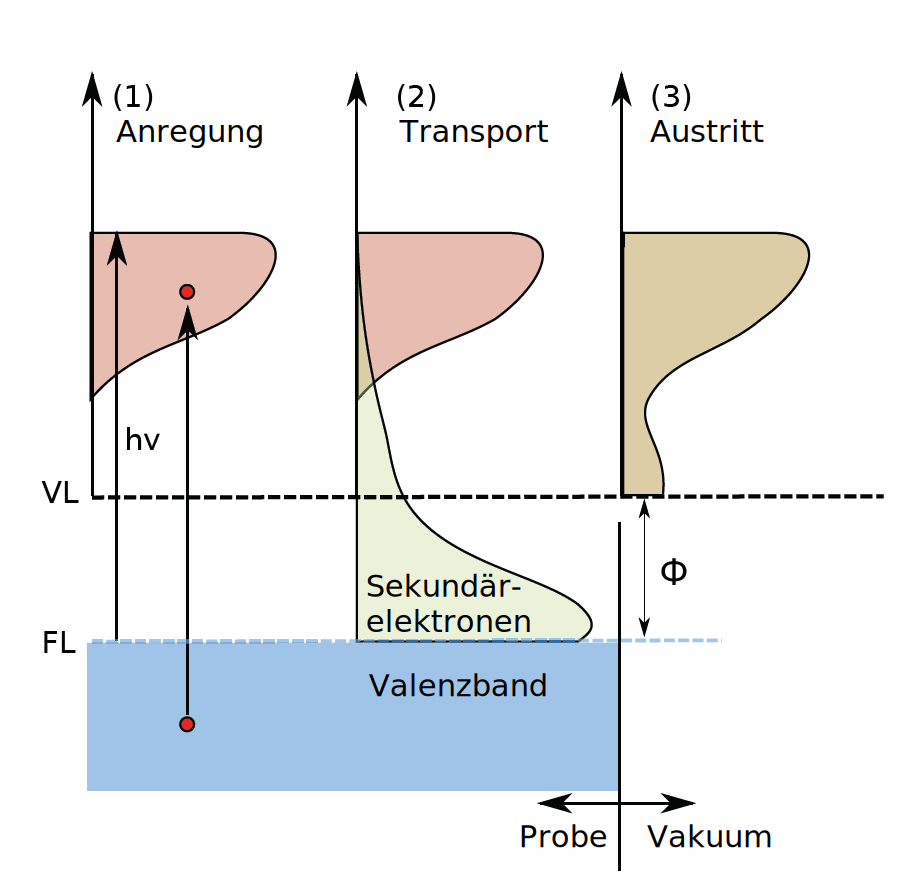
\includegraphics[width=0.6\textwidth]{./content/pictures/3Stufen}
            \caption{Schematische Darstellung des drei Stufen Models für den photoelektrischen Effekt.
            Bestehend aus (1) Absorption, (2) Transport zur Oberfläche und (3) Austritt aus der Oberfläche.
            Kopiert und modifiziert aus~\cite{zhang_synchrotron_2018}.}
            \label{fig:3Stufen}
        \end{figure}
        Dieser Prozess der Emittation eines Elektrons nach Einfall eines Photons lässt sich in einem drei Stufen Model erklären.
        Das Model ist in \autoref{fig:3Stufen} schematisch zu sehen.
        Der erste Schritt ist die Absorption des Photons, wodurch das Elektron angeregt wird. 
        Dieses kann dann innerhalb des Festkörpers zur Probenoberfläche wandern.
        In diesem zweiten Schritt kommt auch die mittlere freie Weglänge der Elektroen zu tragen, weshalb die Methode oberflächensensitiv ist.
        Im dritten Schritt verlässt das Elektron die Oberfläche und wird auf Grund fehlender periodischer Strukturen gebeugt.
        Hier ist die Periodizität des Festkörpers gebrochen, wodurch die senkrechte Komponente des Impulsvektors nicht erhalten bleibt.
        Dahingegen bleibt der Impulsvektor parallel zur Oberfläche $k_{||}$ erhalten.

        \begin{figure}
            \centering
            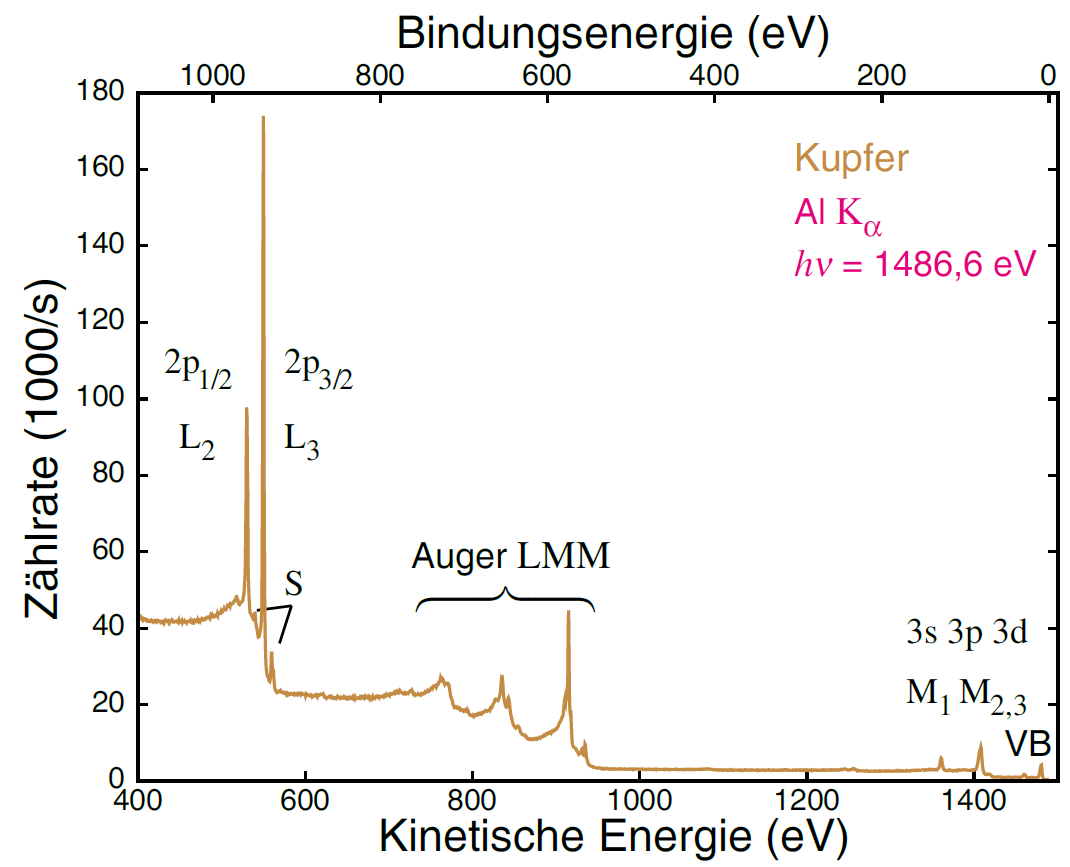
\includegraphics[width=0.6\textwidth]{./content/pictures/Band}
            \caption{Ein Photoemissionsspektrum von Kupfer.
            Im niedrigen Bindungsenergiebereich befindet sich das Valenzband. 
            Zu höheren Bindungsenergien treten dann die Kernniveaus in den Vordergrund, gemeinsam mit den Augerelektronen-Peaks und satelliten-Linien.
            Aus~\cite{Fauster}.}
            \label{fig:Band}
        \end{figure}
        Ein beispielhaftes Spektrum ist in \autoref{fig:Band} zu finden.
        Die Fermikante, bis wohin alle Zustände besetzt sind ist im Spektrum nicht zu erkennen, legt allerdings die Bindungsenergie \SI{0}{\electronvolt} fest.
        Im niederenergetischen Bindungsenergiebereich handelt es sich um Zustände des Valenzbandes zu höheren Energien treten dann Zustände der Kernniveaus auf.
        Zusätzlich treten auch diskrete Linien auf, die durch Augerelektronen hervorgerufen werden.
        Diese Augerelektronen besitzen immer eine feste kinetische Energie, da sie durch den Übergang zwischen zwei Schalen stammen und somit unabhängig von der verwendeten Photonenenergie.
        Zum Ende des Spektrums nimmt der Untergrund stetig zu, was durch inelastisch gestreute Elektronen zustande kommt.
        Nach jedem Peak steigt der Untergrund stufenartig an, da vermehrt Elektronen für die Streuung bereitstehen.
        Im Bereich der niedrigen kinetischen Energie nimmt dieser Effekt ein Maximum an, die Sekundärelektronen.
        Zusätzlich im Spektrum sind Satelieten (S) zu sehen, diese stammen von der nicht ganz monochromatischen Photonenstrahlung. %Übergang von Elektronen bei mehrfachionisierten Atomen.

        Je nach Energie der verwendeten Photonen lässt sich in maßgeblich zwei Bereiche unterscheiden.
        Zum Einen in den Bereich der Röntgenstrahlung (\textit{X-Ray}), womit kernnahe Zustände untersucht werden.
        Zum Anderen den Bereich der ultravioletten Strahlung, hier können Zustände nahe der Fermikante sichtbar gemacht werden.
        Die verschiedenen Energiebereich sind notwendig, damit die angeregten Elektronen eine kinetische Energie im oberflächensensitiven Bereich haben.
        Diese erste Methode wird XPS genannt, wohingegen die zweite Methode mit UPS abgekürzt wird.

        \subsection{Röntgenphotoelektronenspektroskopie - XPS}
            In den Energiebereich der weichen Röntgenstrahlung fallen Photonen mit einer Energie von \SIrange{0.1}{10}{\kilo\electronvolt}~\cite{Fauster}.
            Diese Energien sind nur mit klassischen Röntgenquellen oder einem Synchrotron erreichbar.
            Solche hohen Energien sind notwendig um Elektronen aus Kernniveaus anzuregen.
            % Die kernnahen Niveaus sind schwieriger zu beeinflussen und eigenen sich besonders gut zur Elementanalyse.
            Mit dieser Methode lässt sich ebenfalls die chemische Zusammensetzung untersuchen.
            Leicht unterschiedliche Positionen für verschiedene Ionisationszustände und Bindungszuständen können dabei Rückschlüsse auf chemische Umgebungen zulassen.
            So verschiebt sich die Energie auch, je nach dem ob die Atome an der Oberfläche oder tiefer im Festkörper sind von denen die Elektroen emittiert werden.

            Ein einzelnes so detektierte Merkmal unterliegt dabei mehrern Effekten. 
            Die Breite des charakteristischen Merkmals wird durch die Energiebreite der verwendeten Photonen und der Auflösung des Detekters beschränkt.
            Hinzu kommen thermische Verbreiterungen, weswegen bessere Energieauflösungen erreicht werden, wenn die Probe gekühlt wird.
            % Hinzukommen thermische Verbreiterung, sowie 
            Nach der Entflatung durch alle anderen Merkmal verbreiternden Effekte ergibt sich die die Lebensdauer des Endzustandes, welche antiproportional zur Linienbreite ist.
            Einseitige Verbreiterungen treten durch inelastische Streuungen der Photoelektronen auf.

            Hinzukommt, dass sich einzelne Linien als Dubletts ausbilden.
            Dies rührt von der Spin-Bahn-Kopplung also der Aufspaltung auf Grund des Spins.
            Ihre Intensitätsverhältnisse ergeben sich aus ihrem Entartungsgrad. 
            Ein Beispiel stellen die $\text{L}_2$- und $\text{L}_3$-Linien in \autoref{fig:Band} dar.
            Die Intensitäten der $\text{M}_{1,2,3}$ sind deutlich geringer, da ihr Wirkungsquerschnitt für die Anregung mit der Photonenenergie von \SI{1486.6}{\electronvolt} geringer ausfällt.
        
        \subsection{Röntgenabsorptionspektroskopie - XAS}
            Für die Durchfürung von Röntgenabsorptionsmessungen ist eine durchstimmbare Photonenquelle im weichen Röntgenbereich notwendig.
            Dies ist aktuell nur durch Synchrotrons und Freielektronenlaser realisierbar.
            Hierbei wird die Photonenenergie $h\nu$ über einen bestimmtren Bereich verriert. % in der eine Abosrptionskante liegt abgetastet.
            Trifft ein Photon auf die Oberfläche so wird dieses absorbiert und kann ein Photoelektron auslösen.
            Wie viele Photonen diesen Prozess anregen können hängt davon ab, ob sich Elektronen bei der Energie $h\nu = E_\text{B}+\Psi$ befinden.
            Energien an den schlagartig die absorption steigt werden auch Absorptionskanten genannt und sind charakteristisch für verschiedene Elemente. 
            Es handelt sich dabei dann um einen Übergang aus einem bestimmten kernnahen Zustand in einen unbestzten Zustand.
            Durch die Wahl der Polarisation des Lichtes kann auch spinsensetiv selktiert werden, welche Elektronen ausgelöst werden.

            Wird die Absorprionskante feiner aufgelöst so lassen sich Oszillationen erkennen.
            Diese rühren daher, dass die emittierten Elektronen an Nachbaratomen streuen und zurück zum emittierenden Atom gestreut werden.
            Hier beeinflussen diese dann die Wellennatur des Elektrons und es kommt zu konstruktiver und destruktiven Interferenzen~\cite{Fauster}.
            Je nach kinetischer Energie der emittierten Elektronen müssen dabei nur nächste Nachbarn oder auch weiter entfernte Nachbarn berücksichtigt werden.
            
            Neben der Abhänigkeit von der Photonenenergien ist die Absorption auch von der Polarisation des Lichts selbst abhängig.
            So lässt sich aus den Unterschieden der Absorptionsintensitäten für s- und p-polarisiertem Licht die Neigung von Molekülen auf der Oberfläche kalkulieren\cite{floreano_periodic_2008}.
            Für zirkularpolarisiertes Licht ergibt sich aus dem Intensitätsunterschied der links- und rechtszirkularpolarisertem Licht die Magnetisierung~\cite{stohr_magnetism_2006}.

        \subsection{Ultraviolettphotoelektronenspektroskopie - UPS} \label{sec:UPS}
            Die ultraviolette Strahlung besitzt eine Energie der Photonen im Bereich von \SIrange{10}{1000}{\electronvolt}~\cite{Fauster}.
            Photonen in diesem Energiebereich können auch in Laboren mit Gasentladungslampen erzeugt werden, sind aber ebenfalls an Synchrotrons verfügbar.
            Diese Energien eignen sich besonders gut für Zustände nähe der Fermikante, also auch den Oberflächenzuständen.
            In diesen Bereich fallen auch die Energien die zur Molekülorbital Tomographie genutzt werden, welche in \autoref{sec:MOT} eingeführt wird.

            Es können somit Elektronen aus dem Valenz- und Leitungsband angeregt und emittiert werden. 
            Auf Grund der geringen Photonenenergie können damit keine stark gebundenen Zustände wie die Rumpfniveaus untersucht werden.
            Hier werden Elektronen aus ihrem Anfangszustand $\Psi_\text{i}$ (i = \textit{intinal}) mit der Energie $E_\text{i}$ und mit $N$ Elektronen gefüllt ist, in einen höheren Zustand $\Psi_\text{f}$ (f = \textit{final}) mit der Energie $E_\text{f}$  angeregt.
            Der höher liegende Energie Zustand kann nur erreicht werden, wenn die eingestrahlte Photonenenergie dafür ausreicht.
            So ergibt sich nach Fermis goldenen Regel die Übergangswahrscheinlichkeitsmatrixelmente
            \begin{equation}
                I_\text{fi} \propto \frac{2\pi}{\hbar} \abs{\bigl<\Psi_\text{f}|\Delta|\Psi_\text{i}\bigr>}^2 \, \delta\left(E_\text{f}-E_\text{i}-h\nu\right).
                \label{eqn:Fermi_gold}
            \end{equation}
            Sie enthälen den Polarisationsfaktor $\Delta \approx \frac{\symup{e}\hbar}{m}\vec{A}\cdot\vec{\nabla}$, welcher die Interaktion mit dem Photonenfeld berücksichtigt.
            Dabei beschreibt $\vec{A}$ das klassische Vektorpotential des externen elektrischen Feldes~\cite{cao_theory_2010}.


        \subsection{Winkelaufgelöste Photoelektronenspektroskopie - ARPES} \label{sec:ARPES}
            Bisher wurde  auf den Austrittswinkel der Elektronen nicht genauer eingegangen, zumal bei XPS und UPS auch egal ist unter welchem Winkel die Elektronen die Probe verlassen.
            Diese Messungen werden meist auch in normaler Emission, also parallel zur Oberflächennormalen, vermessen.
            Über alle Austrittswinkel gemittelten Spektren werden auch als integrierte Spektren bezeichnet.
            \begin{figure}
                \centering
                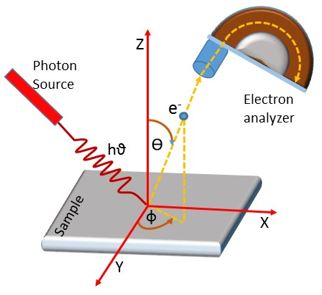
\includegraphics[width=0.5\textwidth]{./content/pictures/ARPES}
                \caption{Versuchsanordnung zur Messung winkelaufgelöster Photoemissionsspektren. Aus~\cite{ARPES}.}
                \label{fig:ARPES}
            \end{figure}

            Die genaue Winkelverteilung der Elektronen wird bei der winkelaufgelösten Photoelektronenspektroskopie genauer untersucht.
            Hierzu wird vom Analysator nur ein kleiner Winkelbreich akzeptiert und der Winkel zwischen Probe und Analysator stets varriert.
            Schematisch ist dies auch in \autoref{fig:ARPES} dargestellt.
            Für jede Winkelkombination aus polarem $\theta$ und azimunthalen $\phi$ Winkel wird ein UPS Spektrum aufgezeichnet.
            Die entsprechenden Impulsvektoren lassen sich aus den Winkeln und der kinetischen Energie nach
            \begin{gather}
                k_\text{x} = \sqrt{\frac{2 \text{m}_\text{e} E_\text{Kin}}{\hbar^2}} \sin\theta \cos\phi \\
                k_\text{y} = \sqrt{\frac{2 \text{m}_\text{e} E_\text{Kin}}{\hbar^2}} \sin\theta \sin\phi
            \end{gather}
            berechnen~\cite{MM_4}.
            Wird für eine feste Energie über alle Winkel integriert und dies für jede gemessene Energie aufgetragen ergibt sich eine integriertes Spektrum.
            Dies hat die Bezeichnung \textit{electron density curve} (EDC), da sie die Zustandsdichte des Valenzbandes wiederspiegelt.

            Von der Seite der Theorie wird das ein Stufen Model der Photonelektronenemission verwendet, welches den Prozess der Photoemission besser beschreibt, aber nicht so anschaulich wie das drei Stufen Model ist.
            Es berücksichtigt unter Anderem, den Austrittswinkel der Elektronen (polar $\theta$ und azimuthal $\phi$) sowie den finale Zustand $\Psi_\text{f}$ mit einer Energie $E_\text{Kin}$.
            So ergibt sich die Photoelektronenintensität in entsprechende Richtung 
            \begin{equation}
                I(\theta, \phi, E_\text{Kin}) \propto \sum_i \abs*{\bigl<\Psi_\text{f}(\theta, \phi, E_\text{Kin})|\vec{A}\cdot\vec{p}|\Psi_\text{i}\bigr>}^2 \times \delta\left(E_\text{i}+E_\text{Kin}+\Phi-h\nu\right))
            \end{equation}
            vom Anfangszustand $\Psi_\text{i}$ in der Dipolapproximation~\cite{MM_2}.
            Durch die ebene Wellen Approximation des Endzustands ist der Photoelektronenstrom proportinal zur Fouriertransformation des Anfangszustandes.
            So ergibt sich unter Beachtung des Polarisationsfaktors $\abs*{\tilde{\Psi}_\text{i}(\vec{k})} \propto \frac{\sqrt{I_\text{i}(\theta, \phi)}}{\abs*{\vec{A}\cdot\vec{k}}}$.

    \section{2D Photoelektronen Mikroskopie} \label{sec:2D-PES}
        Die 2D Photoelektronen Mikroskopie ist eine sehr viel versprechende Technik, die für immer mehr Aufsehen in den letzten Jahren gesorgt hat.
        Der größte Vorteil liegt wohl in der Kombination von spektroskopischen Methoden und mikroskopischen Methoden.
        Zuerst wurde dies 1933 durch E. Brüche entdeckt, der eine Zinkplatte mit Hilfe von Photoelektronen und einer magnetischen Linse auf einem Leuchtschirm abbildete~\cite{bruche_elektronenmikroskopische_1933}.
        Sie nutzt die Prinzipien der Energie- und Impulserhaltung um Bilder der Proben im Realraum oder Impulsraum aufzulösen.

        \begin{figure}
            \centering
            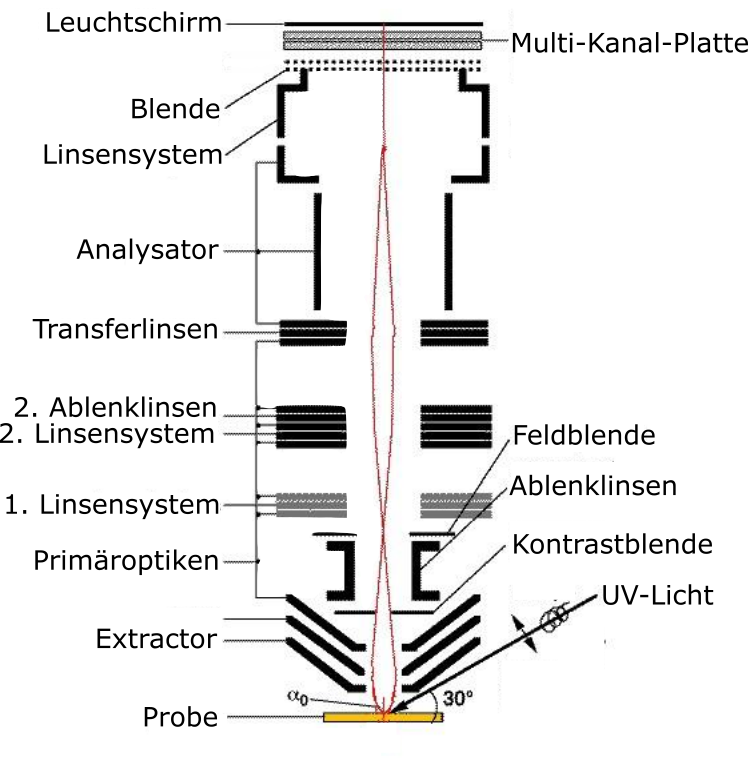
\includegraphics[width=0.6\textwidth]{./content/pictures/PEEM_schemaneu.png}
            \caption{Vereinfachter Aufbau eines 2D Photoelektronen Mikroskopes. Vorlage aus~\cite{KUCH}, modifiziert.}
            \label{fig:MM}
        \end{figure}
        Ein exemplarischer Aufbau ist in \autoref{fig:MM} zu sehen.
        Die durch die Photonen angeregten Elektronen werden durch ein starkes elektrisches Feld von einigen \si{\kilo\volt} von der Probe zum Analysator hin beschleunigt.
        Das Extractorfeld kann bis auf \SI{29}{\kilo\volt} erhöht werden, wird standardmäßig aber auf \SI{10}{\kilo\volt} festgesetzt.
        Durch diese große Spannung zwischen Probe und Extraktor ist es möglich einen großen Sichtbereich im Impulsraum abzudecken.
        Dies ist nötig, da durch den streifenden Einfall der Photonen und der Abberation der elektrostatischen Linsen nur einen kleinen Akzeptanzwinkel zur Verfügung stehen würde.
        Wichtig bei der Kathoden Linse ist, dass das Feld zwischen Probe und Linse sehr homogen ist, damit der Austrittswinkel erhalten bleibt, dies hat zur Folge, dass die Probe auch eine möglichst ebene Oberfläche aufweisen muss.
        Anschließend werden die Elektronen durch elektrostatische Linsen fokussiert und durch die einzelnen Blenden geleitet.
        Sie sind so konzipiert, dass die Bildebene und die hintere Brennebene immer an der selben Position, der Blenden bleiben.
        Je nach dem an welcher Stelle eine Blende eingesetzt wird ergibt sich ein Bild im Realraum oder im Impulsraum.
        Damit der Spot auch immer im Zentrum der Blenden liegt gibt es im Linsensystem noch elektrostatische Verschiebungslinsen, welche den Strahl ablenken.

        Nach den Blenden folgt ein weiters Linsensystem aus elektrostatischen Linsen, welche das Bild auf den Ausgang des Linsensystems fokussieren.
        Hier befinden sich zwei magnetische Verschiebungslinsen um Drift zu korrigieren.
        Im Anschluss gehen die Elektronen in ein Transferlinsensystem über, welches dafür sorgt, dass ein einszueins Abbild auf die Eingangsblende des Analysators trifft.
        Die Eingangsblende kann in ihrer Größe varriert werden, sodass nur ein Teil der Elektronen in den Analysator eintreten.
        Je kleiner die Blende gewählt wird, desto besser ist die Energieauflösung aber so kleiner die Gesamtintensität.
        Als Energiealysator kommt ein hemisphärischer Analysator zum Einsatz.
        Bei dem hemisphärischer Analysator werden die Elektronen zwischen zwei Halbkugeln durch ein statisches elektrisch Feld auf eine Kreisbahn gezwungne.
        Dabei ist das Feld so gewählt, dass nur die mit der richtigen kinetischen Energie eintretenden Elektronen auch auf die Austrittsblende abgebildet werden.
        Ferner wird der Analysators so eingestellt, dass Elektronen mit einer Energie von \SI{50}{\milli\electronvolt} um die eingestellte Energie den Analysator passieren können, dies ist die Pass-Energie.
        
        Nach dem Detektor gibt es eine weiter Linseneinheit, welche zusammen mit einer Blende das gewünschte energieaufgelöst Bild auswählt und es auf die Detektorgröße aufweitet.
        Anschließend durchlaufen die Elektronen eine Mikrokanalplate (eine Art Elektronenvervielfacher) und prallen auf den Phosphorschirm, der an den entsprechenden Stellen aufleuchtet.
        Durch die Kamera wird dieses Leuchten regestriert und das räumliche oder rekrusives Bild kann rekostruiert werden~\cite{SPECS-MM}.
        Bei dem Detektor handelt es sich um eine CMOS Kamera die das Bild der auf den Leuchtschirm auftreffenden Elektronen aufnimmt.
        CCD (\textit{Charge Coupled Device}) Detektoren sind ein Standard bei ARPES Messungen, sie integrieren die analoge Photonenintensitäten oder einzelne Lichtblize werden aufgezeichnet.
        Einer der Nachteile ist die geringe Abtastrate auf Grund der hohen Erholungszeit.
        Hier wird allerdings eine CMOS (\textit{Complemantary metal-oxid-semiconductor}) Kamera verwendet.
        Dabei wird ein einzelnes Bild in nur wenigen Millisekunden erfasst, dies ist durch die Kombination von Kamera und Grafigprozessor möglich.
        Der Vorteil der CMOS Kamera Technik gegenüber der klassischen CCD  Kamera Technik ist, die Erfassung der wahren Pulszählraten~\cite{CMOS}.
        
        Es gibt zwei verschiedene Betribsmodi welche ferner erläutert werden.
        \begin{figure}
            \centering
            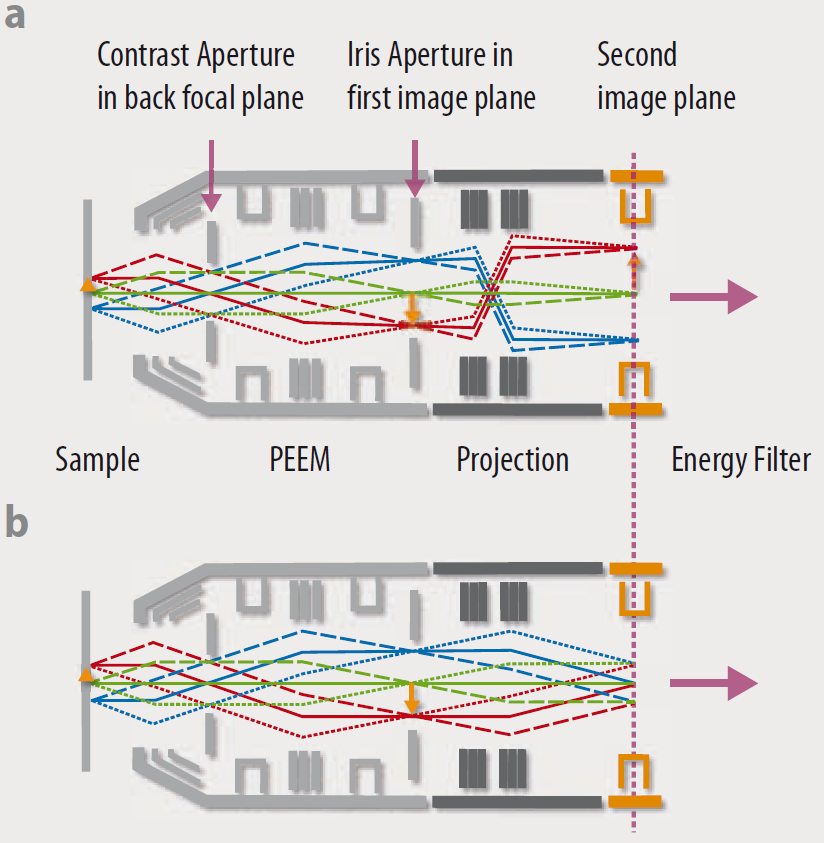
\includegraphics[width=0.5\textwidth]{./content/pictures/Real_k.PNG}
            \caption{Die verschiedenen Konfiguration der Blenden um zwischen Realraum und Impulsraum Bild umzuschalten. Aus~\cite{Focus}.}
            \label{fig:real_k}
        \end{figure}
        Für den Impulsraum ist dies in \autoref{fig:real_k}\,a und für den Realraum in \autoref{fig:real_k}\,b dargestellt.
        Vorteil der Umschaltung zwischen den Modis ist, dass auf sehr kleinen Bereichen die im Realraum bestimmt wurden dann auch Messungen im reziproken Raum durchgeführt werden können.


        \subsection{Impulsraum Aufnahmen}
            Um ein Bild im Impulsraum aufzunehmen wird die Blende im der Bildebene eingefahren, die so genannte Feldblende (\textit{field aperture}).
            Durch die Blende wird ein Ausschnitt auf der Probe ausgwählt, von der die emittierten Elektronen erfasst werden.
            Bei einem Blendendurchmesser von \SI{20}{\micro\meter} und der Vergrößerung (\textit{magnification}) von~\num{5} ist der ausgewählt Bereich etwa \SI{4}{\micro\meter} groß.
            Bei der Aufnahme im Impulsraum wird bei der gesamten Abbildungsoptik der Austrittswinkel erhalten.
            So wird auf die Eintrittsblende des Analysators das Beugungsbild abgebildet.
            Das verwendete Mikroskop kann einen Austrittswinkel von biszu $\pm\SI{90}{\degree}$ erfassen für eine Energie kleiner als \SI{50}{\electronvolt}~\cite{SPECS-MM}.
            Für größere kinetische Energien wird das Sichtfeld auf $\pm\SI[per-mode=reciprocal]{3.6}{\per\angstrom}$ beschränkt.
            Dabei spielt es keine Rolle wo auf der Probe die Elektronen emittiert werden.

            Dies wird auch Impuls Mikroskopie (\textit{Momentum Microscopy}) genannt.
            Bei der Impuls Mikroskopie ist die zeitgleich Erfassung des polaren und azimuntalen Austrittswinkel von großer Bedeutung. 
            So entsteht durch die zusätzlich Sortierung der Elektronen nach ihrer kinetsichen Energie ein dreidimensionaler Datensatz.
            Wird über das gesamte Bild also alle Winkel integriert so ergibt sich die Kurve der Elektronendichte (EDC, \textit{electron density curve}).
            Sie ist vergleichbar mit der Zustandsdichte.

        \subsection{Realraum Aufnahmen}
            Es ist ferner möglich Bilder im Realraum aufzunehmen.
            Dies geschieht durch Einsetzen einer Blende in dem hinteren Brennpunkt, die Kontrastblende (\textit{contrast aperture}).
            Dabei können sehr kleine Spots von \SIrange{50}{200}{\micro\meter} ausgewählt werden.
            Um den Kontrast im Bild zu erhöhen werden nur Elektronen mit einem bestimmten Austrittswinkel für die Erstellung des Bildes erfasst.
            Mit Hilfe der Kontrastblenden kann dann eine Auflößung von einigen \si{\nano\meter} erreicht werden \textbf{QUELLE}. 
            Auf dem Eintrittsspalt des Energyanalysators wird dann das Bild der Oberfläche projeziert.
            Das Bild wird bei festen Energiefilter-Einstellungen aufgenommen.
            Der Modi wird auch als PEEM (\textit{Photon emitted electron microscopy}) bezeichnet.

        \subsection{Erweiterungen}
            Als Erweiterung der 2D Photoelektronen Mikroskopie sind auch zeitaufeglöste Messungen möglich.
            Hierbei erfolgt die Anregung mit zwei zeitlich versetzten Pulsen. 
            Dabei regt der erste Puls die Elektronen in einen höheren Zustand an und der zweite Puls löst diese dann aus.
            So ist es auch möglich zuvor unbesetzte Zustände (zwei Photonenemission) zu untersuchen.
            Wird der zeitliche Versatz zwischen den beiden Pulsen varriert so ist auch die Lebensdauer der Zustände abschätzbar.
            Für die gepulste Photonenquellen würde sich ein Flugzeit (TOF, \textit{Time of flight}) Analysator besser eignen.
            In einem TOF Analysators wird die kinetische Energie aus der Flugzeit der Elektronen bestimmt, weswegen es nur für gepulste Photonenquellen möglich ist.
            Der Vorteil liegt darin, dass direkt ein ganzer Datensatz für alle Impuls- und Energiewerte erfasst werden kann.

            Mögliche Erweiterung wäre auch die Elektronen nach der Energieselection auch noch nach ihrem Spin zu sortieren.
            So lassen sich dann auch die magnetischen Eigenschaften genauer veranschaulichen.
        
    \section{Molekül Orbital Tomographie} \label{sec:MOT}
        Die Molekül Orbital Tomographie vereinigt nun die Vorteile der Impulsmikroskopie mit der Theorie der Dichtefunktionaltheorie (DFT) um Molekülorbitale zu identifizieren.
        Aus der Theorie können die Orbitale der Moleküle in der Gasphase im Realraum berechnet werden~\cite{database}.
        Werden diese dann Fourier transformiert, so ergibt  die Aufenthaltswahrscheinlichkeiten der Elektronen abhängig von ihrem Impuls.
        Nun können die Moleküle bei einer bestimmten kinetischen Energie geschnitten werden und es ergibt sich ein zweidimensionales Bild~\cite{brandstetter_kmappy_2021}.
        Ferner kann auch die Wechselwirkungswahrscheinlichtkeit mit der verwendeten Photonenenergie berücksichtigt werden.
        Aus Messungen im Impulsraum können dann durch einen Vergleich die Molekülorbitale zugeordnet werden.
        Dies ist nur möglich, wenn sich die Moleküle ordnen wie z.B. auf einigen metallischen Oberflächen.

        Wie bereits in \autoref{sec:ARPES} erwähnt ist der Photoelektronenstrom in der Approximation einer ebenen Welle des Endzustands durch die Fouriertransformation des Anfangszustands verknüpft.
        So kann also durch erneute Fouriertransformation aus dem Impulsraum zurück in den Realraum auf die Molekülorbitale geschlossen werden~\cite{MM_2}.

        Unter der Beachtung von: (i) der Emission von $\pi$-Orbitalen großer Moleküle, (ii)~dass der Winkel zwischen Polarisationsvektor $\vec{A}$ und Richtung der austretenden Elektronen $\vec{k}$ klein ist und (iii) die Molekühle aus leichten Atomen bestehen, ist es möglich mit der Annahme der ebenen Welle und DFT die Molekülstruktur im Realraum zu berchnen \cite{MM_2}.
        \begin{figure}
            \centering
            \begin{subfigure}{0.3\textwidth}
                \centering
                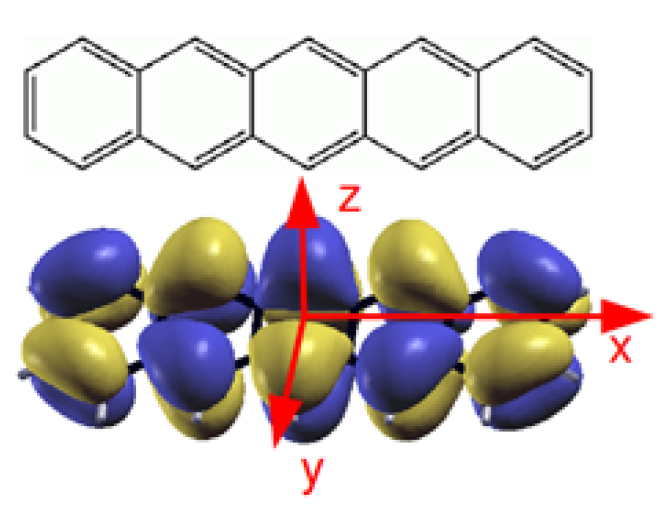
\includegraphics[width=0.9\textwidth]{./content/pictures/DFT1.PNG}
                \caption{}
                \label{fig:DFT1}
            \end{subfigure}
            \begin{subfigure}{0.3\textwidth}
                \centering
                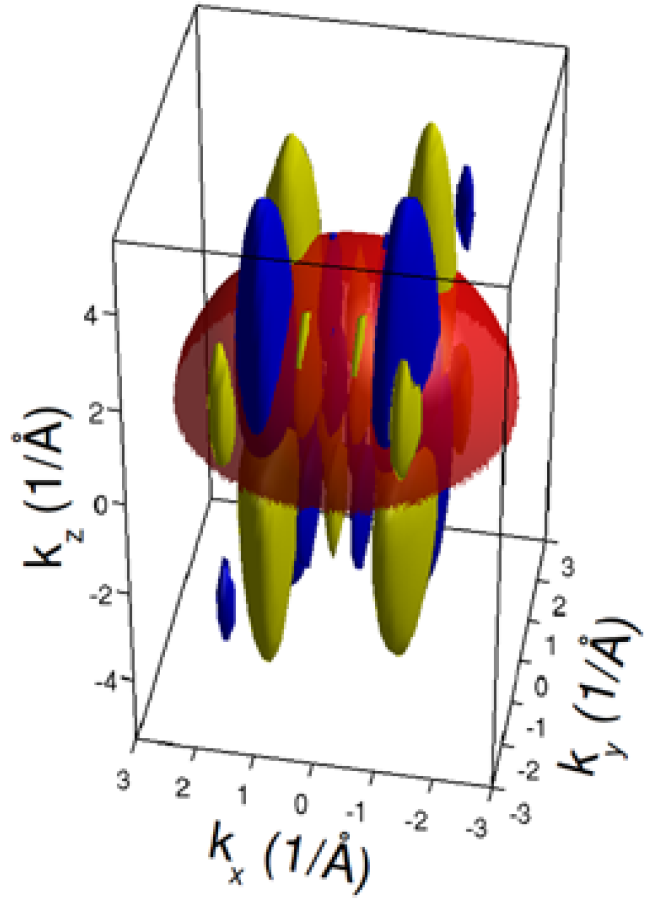
\includegraphics[width=0.9\textwidth]{./content/pictures/DFT2.PNG}
                \caption{}
                \label{fig:DFT2}
            \end{subfigure}
            \begin{subfigure}{0.3\textwidth}
                \centering
                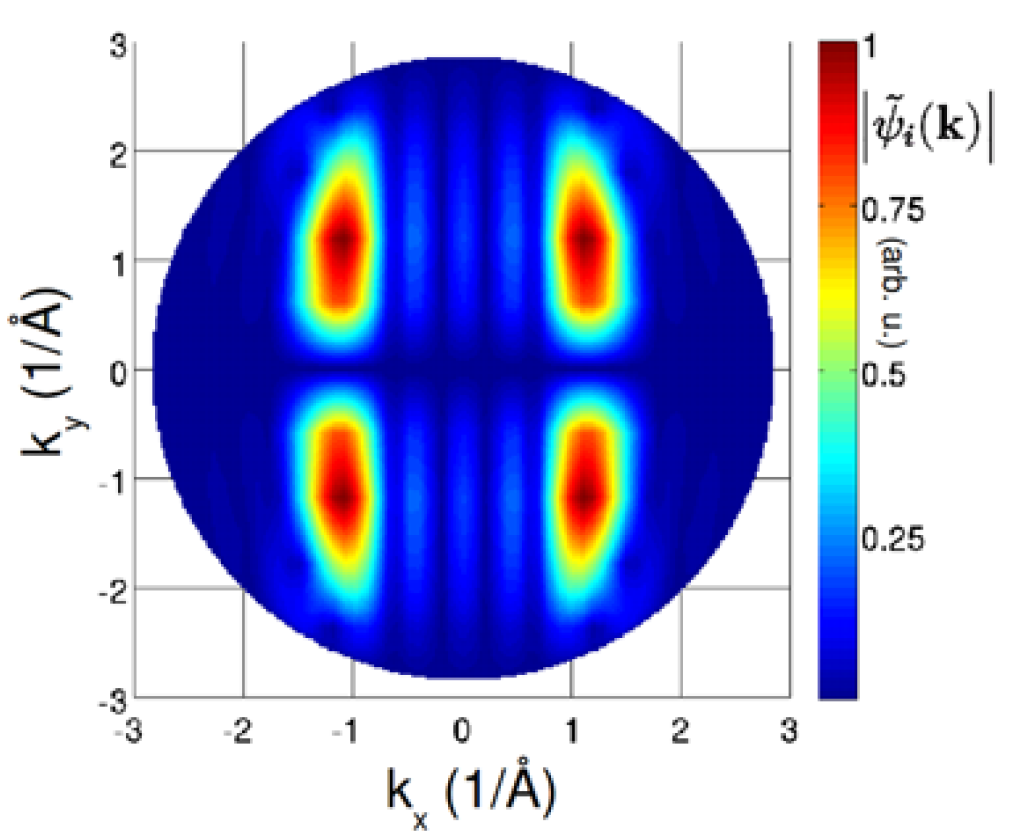
\includegraphics[width=0.9\textwidth]{./content/pictures/DFT3.PNG}
                \caption{}
                \label{fig:DFT3}
            \end{subfigure}
            \caption{In \subref{fig:DFT1} ist die sich aus der Dichtefunktionaltheorie (DFT) ergebene Struktur von Pentacene gezeigt.
            Die durch Fouriertransformation gewonnen Orbitalstruktur im reziproken Raum \subref{fig:DFT2}.
            \subref{fig:DFT3} die Projektion der Fouriertransformation der Molekülorbitale für eine feste kinetische Energie.
            Aus~\cite{MM_2}}
            \label{fig:DFT}
        \end{figure}
        Dies ist beispielhaft in \autoref{fig:DFT1} für Pentacene geschehen.
        Wird nun eine Fouriertransformation durchgeführt ergibt sich das Bild \autoref{fig:DFT2}.
        Schließlich wird die Fouriertransformation entlang einer Ebene konstanter kinetischer Energie, was der roten Hemisphäre in \autoref{fig:DFT2} entspricht, geschnitten.
        Es ergibt sich die Projektion in \autoref{fig:DFT3}.
        Nun kann diese Projektion mit der gemessenen Photoelektronenintensitäten verglichen werden.

        Mit Hilfe der Molekülorbitaltomographie ist es nicht nur möglich Merkmale im Valenzband einzelnen Molekülorbitalen zuzuordnen, sondern auch ihre Ausrichtung auf dem Substraht zu bestimmen.
        So kann zum Beispiel die Neigung der Molekühle in eine Verschiebung der projezierten Molekülorbitalmerkmale in den Impulsbildern enden.
        Auch kann die Ausrichtung der Molekühle entlang der Symmetrien des Substrahtes bestimmt werden.

    \section{Versuchsaufbau}
    \label{sec:Versuchsaufbau}
        \begin{figure}
            \centering
            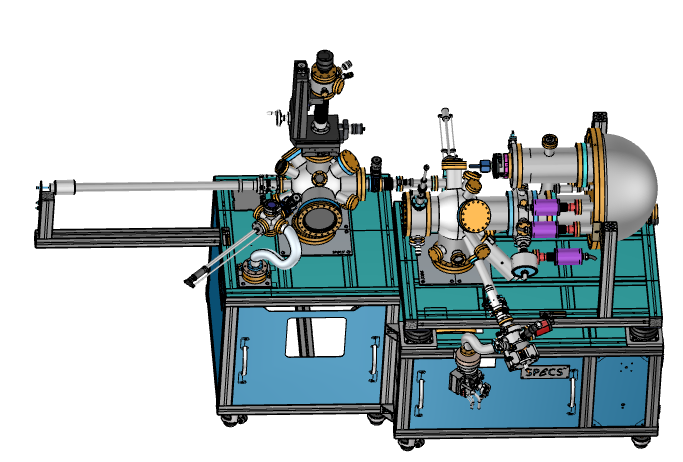
\includegraphics[width=0.7\textwidth]{./content/pictures/MM.png}
            \caption{Der für die durchgeführten Experimente verwendete Aufbau.}
            \label{fig:aufbau}
        \end{figure}
        Um die in dieser Arbeit untersuchten Proben zu präperieren und zu untersuchen wird der Versuchsaufbau in \autoref{fig:aufbau} verwendet.
        Dieser besteht aus einer Präperationskammer (links im Bild) und dem 2D Photoelektronen Mikroskop KREIOS 150MM von SPECS (rechts im Bild).

        Für die Reinigung der Probe steht eine Ionenquelle zur Verfügung, um die Probe mittels ioneninduzierter Zerstäubung zu reinigen.
        Auf dem Manipulator, mit dem die Probe im Ultrahochvakuum verfahren werden kann, ist eine Elektronenstoßheizung montiert um die Probe aufzuheizen.
        Die Präperationskammer ist mit einer LEED-Optik ausgestattet um die Oberflächenbeschaffenheit zu kontrollieren.
        Ferner befindet sich noch ein Leckventil für Sauerstoff sowie Molekül- und Metallaufdampfer an der Kammer.
        
        Vor der Extraktorlinse des 2D Photoelektronen Mikroskopes befindet sich eine 6-Achsen-Piezostage (Hexapod) mit der die Probe in Position gebracht und ausgerichtet werden kann.
        Messungen erfordern eine exakte Ausrichtung der Oberflächennormalen parallel zur Linsenachse und ferner einen Abstand von \SI{4}{\milli\meter} zum Extraktor.
        Mit dieser Positioniereinheit kann die Probe auch auf unter \SI{10}{\kelvin} abgekühlt werden.
        Als Photonenquelle steht eine Helium-Gasentladungslampe bereit, welche größtenteils Photonen der He-I-Linie (\SI{21.22}{\electronvolt}) emittiert~\cite{UVS}.